%%
%% Copyright 2019-2024 Elsevier Ltd
%%
%% This file is part of the 'CAS Bundle'.
%% --------------------------------------
%%
%% It may be distributed under the conditions of the LaTeX Project Public
%% License, either version 1.3c of this license or (at your option) any
%% later version.  The latest version of this license is in
%%    http://www.latex-project.org/lppl.txt
%% and version 1.3c or later is part of all distributions of LaTeX
%% version 1999/12/01 or later.
%%
%% The list of all files belonging to the 'CAS Bundle' is
%% given in the file `manifest.txt'.
%%
%% Template article for cas-dc documentclass for
%% double column output.

\documentclass[a4paper,fleqn]{cas-dc}
\usepackage{kotex}

% If the frontmatter runs over more than one page
% use the longmktitle option.

%\documentclass[a4paper,fleqn,longmktitle]{cas-dc}

%\usepackage[numbers]{natbib}
%\usepackage[authoryear]{natbib}
\usepackage[authoryear,longnamesfirst]{natbib}
\usepackage{tikz}
\usepackage{placeins}  % FloatBarrier 사용
% subsection 경계에서도 float barrier 자동 삽입
\let\origsubsection\subsection
\renewcommand{\subsection}{\FloatBarrier\origsubsection}

%%%Author macros
\def\tsc#1{\csdef{#1}{\textsc{\lowercase{#1}}\xspace}}
\tsc{WGM}
\tsc{QE}
%%%

% Uncomment and use as if needed
%\newtheorem{theorem}{Theorem}
%\newtheorem{lemma}[theorem]{Lemma}
%\newdefinition{rmk}{Remark}
%\newproof{pf}{Proof}
%\newproof{pot}{Proof of Theorem \ref{thm}}

\begin{document}
\let\WriteBookmarks\relax
\def\floatpagepagefraction{1}
\def\textpagefraction{.001}

% 그림 배치 허용 비율 완화
\renewcommand{\topfraction}{0.9}
\renewcommand{\bottomfraction}{0.9}
\renewcommand{\dbltopfraction}{0.9}
\renewcommand{\textfraction}{0.1}
\renewcommand{\floatpagefraction}{0.8}
\renewcommand{\dblfloatpagefraction}{0.8}

% Short title
\shorttitle{LEO 궤도전이에서의 추력 프로파일 분류}

% Short author
\shortauthors{S. Lee}

% Main title of the paper
\title [mode = title]{저궤도 궤도전이 임무를 위한 최적 연속 추력 프로파일의 분류: 파라메트릭 데이터베이스 연구}

% Title footnote mark
% eg: \tnotemark[1]
%\tnotemark[1]

% Title footnote 1.
% eg: \tnotetext[1]{Title footnote text}
%\tnotetext[1]{}

% First author
\author[1]{Suwon Lee}[orcid=0000-0002-6573-6348]

% Corresponding author indication
\cormark[1]

% Email id of the first author
\ead{suwon.lee@kookmin.ac.kr}

% Credit authorship
\credit{Conceptualization, Methodology, Software, Investigation, Writing - Original Draft}

% Address/affiliation
\affiliation[1]{organization={Department of Future Mobility, Kookmin University},
            addressline={77 Jeongneung-ro, Seongbuk-gu},
            city={Seoul},
            postcode={02707},
            country={Republic of Korea}}

% Corresponding author text
\cortext[1]{Corresponding author}

% Here goes the abstract
\begin{abstract}
본 연구는 재사용 우주비행체(ReUSV) 궤적 설계 및 LEO 군집 운용의 요구에 의해 동기 부여된, 저궤도(LEO) 궤도전이 임무에 대한 최적 연속 추력 프로파일의 포괄적 파라메트릭 분석을 제시한다. 2단계 직접 배치법(two-pass direct collocation)을 사용하여 장반축 변화, 궤도경사각 변화, 출발 및 도착 이심률, 전이 지속시간을 포함하는 5차원 구성 공간에 걸친 최적 궤적 데이터베이스를 생성한다---여기서 전이 지속시간은 단일 공전 미만(sub-single-revolution) 전이로 제한되는 자유 최적화 변수로 취급된다. 결과적 추력 프로파일을 단봉형(unimodal, 단일 피크), 쌍봉형(bimodal, 이중 피크), 다봉형(multimodal, 3개 이상 피크)으로 체계적으로 분류한다. 자동 관련성 결정(automatic relevance determination, ARD) 분석을 통해 추력 프로파일 형태를 지배하는 주요 구성 파라미터를 식별한다. 나아가, 고전적 임펄스 기동과 연속 추력 대응물 사이의 정량적 관계를 확립하여, 임펄스 해가 보다 일반적인 연속 최적 해의 극한 사례임을 보인다. 본 연구의 결과는 임무 설계자에게 이심률 궤도를 포함한 궤도전이 기하에 기반하여 최적 추력 프로파일 특성을 예측할 수 있는 지침을 제공한다.
\end{abstract}

% Use if graphical abstract is present
%\begin{graphicalabstract}
%\includegraphics{}
%\end{graphicalabstract}

% Research highlights
\begin{highlights}
\item 이심률 궤도를 포함한 LEO 간 궤도전이를 위한 최적 연속 추력 프로파일의 파라메트릭 데이터베이스 구축
\item 단일 공전 미만 범위 내에서의 전이 지속시간 자유 최적화 변수 처리
\item 추력 프로파일의 단봉형, 쌍봉형, 다봉형 분류
\item 프로파일 형태를 지배하는 주요 파라미터 식별을 위한 5차원 ARD 분석
\end{highlights}

% Keywords
% Each keyword is seperated by \sep
\begin{keywords}
저추력 궤적 최적화(Low-thrust trajectory optimization) \sep 연속 추력 프로파일(Continuous thrust profile) \sep 저궤도 궤도전이(Low Earth orbit transfer) \sep 직접 배치법(Direct collocation) \sep 파라메트릭 연구(Parametric study)
\end{keywords}

\maketitle

% Main text

%%%%%%%%%%%%%%%%%%%%%%%%%%%%%%%%%%%%%%%%%%%%%%%%%%%%%%%%%%%%%%%%%%
\section{서론}\label{sec:introduction}
%%%%%%%%%%%%%%%%%%%%%%%%%%%%%%%%%%%%%%%%%%%%%%%%%%%%%%%%%%%%%%%%%%

% Paragraph 1: ReUSV motivation and importance of continuous thrust
재사용 우주비행체(reusable space vehicle, ReUSV)에 대한 관심 증가는 저궤도(LEO) 궤적 설계에 새로운 요구를 도입하였다 \citep{Baiocco2021,Grantz2011}. 대기권 재진입 후, ReUSV는 운용 고도로 복귀하기 위해 신속한 궤도 상승(orbit-raising) 기동을 수행해야 한다; 반대로, 임무 완료 또는 서비스 플랫폼과의 랑데부를 위해 제어된 궤도 하강(orbit-lowering) 전이가 필요할 수 있다 \citep{Jung2025}. 이러한 단기간의 단일 공전 미만(sub-single-revolution) 기동은 전기추진(EP) 정지궤도 유지에 전형적인 다주회(multi-revolution) 나선궤적과 근본적으로 다르지만, 전이 중 추진제 소모와 열 부하를 최소화하기 위한 연속 추력 최적화의 혜택을 받는다. 동시에, LEO 위성 군집(constellation)의 확산과 EP 시스템의 광범위한 도입 \citep{Lev2019}은 연속 추력 궤적 최적화를 현대 우주 운용의 필수적 역량으로 확립하였다. 이온 스러스터(ion thruster) 및 홀 효과 스러스터(Hall-effect thruster) 등의 EP 시스템은 비추력($I_{sp}$) 2,000초 이상을 제공하지만 추력 수준이 낮으며 \citep{Jahn1968,Goebel2008}, Dawn \citep{Rayman2000}, Hayabusa2 \citep{Tsuda2020}, SMART-1 \citep{Racca2002}, Starlink 군집 \citep{SpaceNews2023} 등의 임무에서 성공적으로 운용되었다. LEO 환경은 지구 편평도에 의한 $J_2$ 섭동의 지배적 영향, 빈번한 식(eclipse) 구간 \citep{Graham2016}, 원형 및 타원 궤도를 포함하는 다양한 전이 기하 \citep{Topputo2014} 등 고유한 도전 과제를 제시한다.

% Paragraph 2: Overview of existing optimization methodologies
저추력 궤적 최적화를 위한 효율적 방법 개발에 광범위한 연구가 수행되었다 \citep{Betts1998,Conway2010}. 직접법(direct method)은 Hermite-Simpson 배치법 \citep{Herman1996,Hargraves1987} 및 Legendre-Gauss-Lobatto 절점을 이용한 유사분광법(pseudospectral method) \citep{Rao2025,Fahroo2002} 등의 이산화 기법을 통해 연속 최적 제어 문제를 유한 차원 비선형 계획법(nonlinear programming, NLP) 문제로 변환한다. 이러한 접근법은 강건한 구속조건 처리와 신뢰할 수 있는 수렴 특성을 제공하며, 적응적 격자 세분화(adaptive mesh refinement) 기법이 계산 효율성을 더욱 향상시킨다 \citep{Patterson2014}. 볼록 최적화(convex optimization) 기법, 특히 무손실 볼록화(lossless convexification)를 이용한 순차 볼록 계획법(successive convex programming, SCP) \citep{Acikmese2013,Blackmore2012}은 다항 시간 복잡도를 보장하고 비선형 솔버에 내재한 국소 최솟값 함정을 회피하는 강력한 대안으로 부상하였다 \citep{Mao2017,Malyuta2022}. 폰트랴긴의 최소 원리(Pontryagin's minimum principle) \citep{Pontryagin1962}에 기반한 간접법(indirect method)은 이론적으로 최적인 해를 제공하지만 초기 공상태(costate) 추정에 대한 민감도가 높으며, 이는 호모토피(homotopy) 및 연속법(continuation technique)의 개발을 촉진하였다 \citep{Bertrand2002,Caillau2012}. 최근에는 공상태 초기화 및 추력 스위칭 구조 예측을 위한 기계학습(machine learning) 접근법이 탐구되고 있다 \citep{Izzo2019,Zaidi2023}. 형상 기반 방법(shape-based method)은 B\'{e}zier 곡선 \citep{Lee2021bezier} 또는 지수 정현파(exponential sinusoid) 등의 해석적 기저 함수로 궤적을 매개변수화하는 또 다른 패러다임을 제공하며, 특히 단기간 전이에 효과적일 수 있다 \citep{Lee2025eucass}. 이러한 방법론적 다양성에도 불구하고, 기존 연구는 주어진 특정 임무 구성에 대한 최적 궤적을 결정하는 순방향 문제(forward problem) 해결에 주로 집중하고 있다.

% Paragraph 3: Research gap - lack of systematic classification
이러한 진전에도 불구하고, 임무 파라미터가 최적 추력 프로파일 특성에 미치는 영향에 대한 체계적 이해는 여전히 부족하다. 최적 연속 추력 궤적은 뚜렷한 형태적 특징을 보인다: 추력 크기 프로파일은 활주(coasting, 무추력) 호로 분리된 다양한 수의 피크를 나타낸다. 이러한 특징은 고전적 임펄스 기동과 밀접하게 연결되어 있다---두 개의 추력 피크를 갖는 쌍봉형 프로파일은 호만 기동(Hohmann maneuver) \citep{Hohmann1960} 등의 2-임펄스 전이에 대응하며, 다봉형 프로파일은 다중 임펄스 전략 \citep{Edelbaum1967}에 대응한다. 그러나 주어진 전이 구성에 대해 어떤 유형의 추력 프로파일이 나타날지 \textit{사전에(a priori)} 예측할 수 있는 체계적 프레임워크는 존재하지 않으며, 특히 ReUSV 임무와 관련된 이심률 궤도 및 단기간 전이를 포함하는 경우 더욱 그러하다. 임무 설계자들은 특정 LEO 간 궤도전이가 단봉형, 쌍봉형, 또는 다봉형 최적 프로파일을 산출할지, 그리고 이심률을 포함한 어떤 궤도 파라미터가 이 결과에 가장 강하게 영향을 미치는지에 대한 정량적 지침이 부재하다.

% Paragraph 4: Research objectives and approach
본 연구는 이심률 궤도를 포함한 LEO 간 궤도전이에 대한 최적 연속 추력 궤적의 포괄적 데이터베이스를 구축하고, 결과적 추력 프로파일의 체계적 분류 및 분석을 수행하여 이 공백을 해소한다. 전이 지속시간은 규정된 범위 내에서 자유 최적화 변수로 취급되며, ReUSV 궤도 복귀 및 랑데부 시나리오에 해당하는 단일 공전 미만 전이로 한정한다. 구체적 목표는 세 가지이다: (1) 직접 배치법을 사용하여 5차원 구성 공간 $(\Delta a, \Delta i, e_0, e_f, T_f)$에 걸친 최적 궤적 해를 생성하고, (2) 피크 특성에 기반하여 추력 프로파일을 단봉형, 쌍봉형, 다봉형의 뚜렷한 유형으로 분류하며, (3) 통계적 분석을 통해 추력 프로파일 형태를 지배하는 주요 궤도 파라미터를 식별한다. 궤도전이 기하와 최적 추력 프로파일 유형 사이의 정량적 관계를 확립함으로써, 본 연구는 임무 설계자가 상세 최적화 수행 전에 최적 해의 일반적 특성을 예측할 수 있는 역량을 제공한다. 나아가, 연속 추력 프로파일 유형과 고전적 임펄스 기동 사이의 대응 관계를 정량적으로 검토하여, 이 두 궤적 설계 패러다임 간의 이론적 연결을 강화한다.

% Paragraph 5: Paper organization
본 논문의 나머지 부분은 다음과 같이 구성된다. Section~\ref{sec:problem}에서는 연속 추력 궤적 최적화 문제를 정식화하고, 임펄스 기동과의 관계를 확립하며, 비용 함수를 정의한다. Section~\ref{sec:methodology}에서는 직접 배치법 방법론, 데이터베이스 구축 전략 및 추력 프로파일 분류 기준을 기술한다. Section~\ref{sec:results_database}에서는 생성된 데이터베이스를 제시하고 추력 프로파일 유형의 분포를 분석한다. Section~\ref{sec:results_geometric}에서는 시간적 프로파일 특성의 기하학적 분석을 제공한다. Section~\ref{sec:discussion}에서는 결과의 물리적 해석과 실용적 시사점을 논의한다. 마지막으로 Section~\ref{sec:conclusions}에서 주요 결론을 요약하고 향후 연구 방향을 제시한다.


%%%%%%%%%%%%%%%%%%%%%%%%%%%%%%%%%%%%%%%%%%%%%%%%%%%%%%%%%%%%%%%%%%
\section{문제 정식화}\label{sec:problem}
%%%%%%%%%%%%%%%%%%%%%%%%%%%%%%%%%%%%%%%%%%%%%%%%%%%%%%%%%%%%%%%%%%

\subsection{연속 추력 궤적 최적화}\label{subsec:continuous_thrust}

연속 추력 LEO 간 궤도전이를 위한 궤적 최적화 문제를 최적 제어 문제로 정식화한다. 우주선의 상태와 역학은 지구 중심 관성(Earth-Centered Inertial, ECI) 좌표계에서 정의한다. 본 정식화는 전이 지속시간을 자유 최적화 변수로 취급하고, 경계 궤도를 고전 궤도요소로 매개변수화하여 다양한 전이 기하에 걸친 체계적 데이터베이스 구축을 가능하게 한다.

\subsubsection{운동방정식}

우주선 상태 벡터 $\mathbf{x} \in \mathbb{R}^6$는 ECI 좌표계에서의 위치 $\mathbf{r} \in \mathbb{R}^3$와 속도 $\mathbf{v} \in \mathbb{R}^3$로 구성된다:
\begin{equation}
\mathbf{x} = \begin{bmatrix} \mathbf{r} \\ \mathbf{v} \end{bmatrix}
\end{equation}

운동방정식은 다음과 같다:
\begin{equation}\label{eq:eom}
\dot{\mathbf{x}} = \begin{bmatrix} \dot{\mathbf{r}} \\ \dot{\mathbf{v}} \end{bmatrix} = \begin{bmatrix} \mathbf{v} \\ \mathbf{a}_{\text{grav}} + \mathbf{a}_{J_2} + \mathbf{a}_{\text{drag}} + \mathbf{a}_{\text{other}} + \mathbf{u} \end{bmatrix}
\end{equation}
여기서 $\mathbf{u} \in \mathbb{R}^3$는 추력 가속도(제어 입력)이며, 각 가속도 항은 다음과 같이 정의된다.

이체 중력 가속도(two-body gravitational acceleration)는 다음과 같다:
\begin{equation}
\mathbf{a}_{\text{grav}} = -\frac{\mu}{r^3}\mathbf{r}
\end{equation}
여기서 $\mu$는 지구의 중력 상수이고 $r = \|\mathbf{r}\|$이다.

지구 편평도를 고려한 $J_2$ 섭동 가속도는 다음과 같다:
\begin{equation}
\mathbf{a}_{J_2} = -\frac{3\mu J_2 R_E^2}{2r^5} \begin{bmatrix}
x\left(1 - \frac{5z^2}{r^2}\right) \\[4pt]
y\left(1 - \frac{5z^2}{r^2}\right) \\[4pt]
z\left(3 - \frac{5z^2}{r^2}\right)
\end{bmatrix}
\end{equation}
여기서 $J_2$는 제2대상 조화 계수(second zonal harmonic coefficient), $R_E$는 지구 적도 반경, $(x, y, z)$는 ECI 위치 성분이다.

대기 항력 가속도는 다음과 같이 모델링한다:
\begin{equation}
\mathbf{a}_{\text{drag}} = -\frac{1}{2}\rho(h) \frac{C_D A}{m} v_{\text{rel}} \mathbf{v}_{\text{rel}}
\end{equation}
여기서 $\rho(h)$는 고도 $h$에서의 대기 밀도, $C_D$는 항력 계수, $A$는 단면적, $m$은 우주선 질량, $\mathbf{v}_{\text{rel}}$은 회전 대기에 대한 상대 속도이다.

$\mathbf{a}_{\text{other}}$ 항은 태양 복사압(solar radiation pressure), 제3체 중력 효과(third-body gravitational effect), 고차 중력 조화 등의 추가 섭동을 포함하며, 임무 충실도 요구사항에 따라 포함 여부가 결정된다.

\subsubsection{제어 입력}

추력 가속도 $\mathbf{u}(t)$는 전기추진 시스템이 생성하는 가속도를 나타내는 제어 입력으로 사용된다. 이 정식화는 궤적 최적화를 특정 추진 시스템 파라미터(추력 크기 및 질량 유량)로부터 분리하여, 결과를 다양한 우주선 구성에 적용할 수 있게 한다.

\subsubsection{경계 조건}

출발 및 도착 궤도는 고전 궤도요소(classical orbital elements)로 지정한다:
\begin{align}
\boldsymbol{\alpha}_0 &= (a_0, e_0, i_0, \Omega_0, \omega_0) \quad \text{(출발 궤도)} \\
\boldsymbol{\alpha}_f &= (a_f, e_f, i_f, \Omega_f, \omega_f) \quad \text{(도착 궤도)}
\end{align}
여기서 $a$는 장반축(semi-major axis), $e$는 이심률(eccentricity), $i$는 궤도경사각(inclination), $\Omega$는 승교점 적경(right ascension of the ascending node), $\omega$는 근지점 편각(argument of periapsis)이다.

출발 및 도착 궤도상의 위치를 나타내는 진근점이각(true anomaly) $\nu_0$와 $\nu_f$는 자유 최적화 변수로 취급한다. 이 정식화는 최적화기가 각 궤도에서의 최적 출발점과 도착점을 결정할 수 있게 한다:
\begin{align}
\mathbf{x}(0) &= \mathbf{x}(\boldsymbol{\alpha}_0, \nu_0) \\
\mathbf{x}(T_f) &= \mathbf{x}(\boldsymbol{\alpha}_f, \nu_f)
\end{align}
여기서 $T_f$는 전이 지속시간을 나타낸다. $T_f$를 지정 파라미터로 고정하는 기존 정식화와 달리, 본 연구에서는 $T_f$를 범위 구속조건을 갖는 자유 최적화 변수로 취급한다:
\begin{equation}\label{eq:tf_bounds}
T_{\min} \leq T_f \leq T_{\max}
\end{equation}
이는 최적화기가 규정된 범위 내에서 에너지적으로 최적인 전이 지속시간을 결정할 수 있게 한다. $T_{\min}$과 $T_{\max}$는 초기 궤도 주기 $T_0 = 2\pi\sqrt{a_0^3/\mu}$의 단위로 표현되며, 단일 공전 미만(sub-single-revolution) 전이로 한정하도록 선택된다(Section~\ref{subsec:configuration}).

\subsubsection{구속조건}

최적화 문제는 다음의 경로 구속조건을 따른다:

\textit{추력 크기 구속조건:} 추력 가속도의 상한이 존재한다:
\begin{equation}
\|\mathbf{u}(t)\| \leq u_{\max}, \quad \forall t \in [0, T_f]
\end{equation}
여기서 $u_{\max}$는 물리적 추진 한계가 아닌 수치적 안전장치(numerical safeguard)로 기능한다. 이 값은 실제 해에서 상한이 거의 활성화되지 않을 만큼 충분히 크게 설정되며(예: $u_{\max} = 1.0$~km/s$^2$), NLP 솔버가 중간 반복 과정에서 물리적으로 비현실적인 가속도 크기를 탐색하는 것을 방지하는 것이 목적이다.

\textit{최소 고도 구속조건:} 대기권 진입을 방지하고 임무 안전을 보장하기 위해, 우주선 고도는 지정된 최소값 이상이어야 한다:
\begin{equation}
\|\mathbf{r}(t)\| \geq R_E + h_{\min}, \quad \forall t \in [0, T_f]
\end{equation}
여기서 $h_{\min}$은 최소 허용 고도이다.

\subsubsection{비용 함수}

비용 함수는 궤도전이에 필요한 제어 노력을 정량화한다. 에너지 기반(이차) 비용 함수를 채택한다:
\begin{equation}\label{eq:cost_function}
J[\mathbf{u}(\cdot)] = \int_0^{T_f} \|\mathbf{u}(t)\|^2 \, dt
\end{equation}
이는 전이 지속시간 $T_f$에 걸친 추력 가속도 제곱의 적분을 나타낸다.

$L^1$ 노름(연료 최적 정식화 $\int \|\mathbf{u}\| dt$) 대신 $L^2$ 노름을 선택한 이유는 다음과 같다. $L^1$ 노름은 일반적으로 최대 추력과 활주 사이의 불연속 스위칭을 갖는 뱅-뱅(bang-bang) 제어 구조를 유도하여 임펄스 기동과 유사한 형태를 보인다. 반면 $L^2$ 노름은 연속 미분 가능한 부드러운 추력 프로파일을 산출하여 직접 배치법에 의한 수치적 최적화를 용이하게 한다. 중요한 점은, $L^2$ 정식화가 추력 집중 영역의 수와 상대적 시간 배치라는 본질적 피크 구조 특성을 보존하면서도 정밀한 스위칭 시간 탐지와 관련된 수치적 어려움을 회피한다는 것이다. 이는 최소 연료 해의 달성보다 추력 프로파일의 형태적 유형 식별이 주된 관심사인 본 연구의 분류 목적에 적합하다.

\subsubsection{최적 제어 문제 기술}

주어진 궤도 구성 $(\boldsymbol{\alpha}_0, \boldsymbol{\alpha}_f)$과 전이 지속시간 범위 $[T_{\min}, T_{\max}]$에 대해, 연속 추력 궤적 최적화 문제는 다음과 같이 기술할 수 있다:
\begin{equation}\label{eq:ocp}
\begin{aligned}
& \underset{\mathbf{u}(\cdot),\, \nu_0,\, \nu_f,\, T_f}{\text{minimize}} & & J[\mathbf{u}(\cdot)] \\
& \text{subject to} & & \dot{\mathbf{x}} = \mathbf{f}(\mathbf{x}, \mathbf{u}, t) \\
& & & \mathbf{x}(0) = \mathbf{x}(\boldsymbol{\alpha}_0, \nu_0) \\
& & & \mathbf{x}(T_f) = \mathbf{x}(\boldsymbol{\alpha}_f, \nu_f) \\
& & & T_{\min} \leq T_f \leq T_{\max} \\
& & & \|\mathbf{u}(t)\| \leq u_{\max}, \quad \forall t \in [0, T_f] \\
& & & \|\mathbf{r}(t)\| \geq R_E + h_{\min}, \quad \forall t \in [0, T_f]
\end{aligned}
\end{equation}
여기서 $J$는 식~\eqref{eq:cost_function}에서 정의된 비용 함수이고, $\mathbf{f}$는 식~\eqref{eq:eom}의 우변을 나타낸다. 결정 변수에는 추력 가속도 프로파일 $\mathbf{u}(t)$, 출발/도착 진근점이각 $\nu_0$ 및 $\nu_f$, 그리고 전이 지속시간 $T_f$가 포함된다.

이 정식화는 출발-도착 궤도 간 궤도요소 차이 $(\Delta a, \Delta i, e_0, e_f)$로 정의되는 궤도 구성을 변화시키면서, 최적화기가 규정된 범위 내에서 에너지적으로 최적인 전이 지속시간을 결정하도록 함으로써 체계적 파라메트릭 연구를 가능하게 한다.

\subsection{임펄스 기동과의 관계}\label{subsec:impulsive_relation}

Section~\ref{subsec:continuous_thrust}에서 제시한 연속 추력 정식화는 임펄스 기동을 극한 사례(limiting case)로 포함한다. 이 관계는 본 접근법에 대한 이론적 정당성과 연속 추력 프로파일 해석에 대한 실용적 통찰을 제공한다.

\subsubsection{임펄스 기동의 수학적 표현}

임펄스 기동은 시각 $t_k$에서의 순간적 속도 변화 $\Delta\mathbf{v}$로 특징지어지며, 디랙 델타 함수(Dirac delta function)를 사용하여 수학적으로 표현할 수 있다 \citep{Lawden1963}:
\begin{equation}\label{eq:impulse_delta}
\mathbf{u}_{\text{imp}}(t) = \Delta\mathbf{v}_k \cdot \delta(t - t_k)
\end{equation}
여기서 $\delta(\cdot)$는 디랙 델타 함수를 나타낸다. $N$-임펄스 궤적의 경우 제어 입력은 다음과 같다:
\begin{equation}\label{eq:n_impulse}
\mathbf{u}_{\text{imp}}(t) = \sum_{k=1}^{N} \Delta\mathbf{v}_k \cdot \delta(t - t_k)
\end{equation}

이 표현은 임펄스 기동이 일반적 연속 추력 정식화의 특수한 경우임을 보여준다. 제어가 이산적 시간 순간에 집중되어 무한대의 크기를 갖지만 유한한 적분값(속도 변화)을 갖는 형태이다.

\subsubsection{해 공간 포함 관계}

연속 추력과 임펄스 궤적 최적화 문제의 해 공간 사이에는 근본적 관계가 존재한다. $\mathcal{S}_{\text{cont}}$를 연속 추력 제어 하의 실현 가능 궤적 집합, $\mathcal{S}_{\text{imp}}$를 $N$-임펄스 제어 하의 실현 가능 궤적 집합이라 하면, 다음의 포함 관계가 성립한다 \citep{Taheri2020}:
\begin{equation}\label{eq:solution_space}
\mathcal{S}_{\text{imp}} \subset \mathcal{S}_{\text{cont}}
\end{equation}

이 관계는 임펄스 기동으로 달성 가능한 모든 궤적이 연속 추력으로도 달성(또는 근사)될 수 있지만, 그 역은 성립하지 않음을 의미한다. 따라서 연속 추력 문제의 최적 비용은 최적 임펄스 해에 의해 상한이 정해진다:
\begin{equation}
J^*_{\text{cont}} \leq J^*_{\text{imp}}
\end{equation}

나아가, 임펄스 수 $N$이 증가함에 따라 적절한 정칙성 조건(regularity condition) 하에서 임펄스 해는 연속 최적 해에 수렴한다 \citep{Prussing2010}.

\subsubsection{추력 프로파일과 고전적 기동의 대응 관계}

해 공간 관계는 연속 추력 프로파일 특성과 고전적 임펄스 기동 사이의 대응 관계를 시사한다:

\begin{itemize}
\item \textit{단봉형 프로파일}(단일 추력 피크)은 단일 임펄스 기동에 대응하며, 주로 단일 궤도 위치에서의 속도 크기 변화가 필요한 전이에서 관측된다.

\item \textit{쌍봉형 프로파일}(이중 추력 피크)은 호만 전이(Hohmann transfer) 등의 2-임펄스 기동에 대응하며, 출발 및 도착 영역에서 추력 집중이 발생한다.

\item \textit{다봉형 프로파일}(3개 이상의 피크)은 이중 타원 전이(bi-elliptic transfer) 등의 다중 임펄스 기동에 대응하며, 큰 궤도 반경비 변화에서 최적이 된다.
\end{itemize}

이 대응 관계는 본 연구에서 제시하는 추력 프로파일 분류 결과를 해석하기 위한 물리적 직관을 제공한다. 연속 최적 해는 임펄스 해를 ``부드럽게(smooth)'' 하면서 그 기본적 구조를 보존하며, 추력 피크는 임펄스 연소 지점에 유사한 위치에서 발생한다.


%%%%%%%%%%%%%%%%%%%%%%%%%%%%%%%%%%%%%%%%%%%%%%%%%%%%%%%%%%%%%%%%%%
\section{방법론}\label{sec:methodology}
%%%%%%%%%%%%%%%%%%%%%%%%%%%%%%%%%%%%%%%%%%%%%%%%%%%%%%%%%%%%%%%%%%

\subsection{2단계 직접 배치법(Two-Pass Direct Collocation Method)}\label{subsec:direct_collocation}

식~\eqref{eq:ocp}에서 정의한 연속 최적 제어 문제를 2단계 직접 배치법(two-pass direct collocation)을 통해 유한 차원의 비선형 프로그래밍(NLP) 문제로 변환한다. 이 혼합 방법은 에르미트-심프슨 배치법(Hermite-Simpson collocation)의 균일 샘플링 장점과 르장드르-가우스-로바토(LGL) 의사 스펙트럼 방법(pseudospectral method)의 높은 정확도를 결합한 것이다 \citep{Hargraves1987,Rao2025,Fahroo2002}.

2단계 접근법의 동기는 의사 스펙트럼 방법의 근본적 한계에서 비롯된다. LGL 노드는 정의역 경계 근처에 밀집되어, 최적 해의 추력 집중 영역(피크)과 일치하지 않을 수 있다. 피크 위치를 \textit{사전에(a priori)} 알 수 없으므로, 먼저 균일 분포 노드로 예비 최적화를 수행하여 추력 프로파일 구조를 파악한 후, 적응적 노드 배치로 정밀 최적화를 수행한다.

\subsubsection{1단계: 에르미트-심프슨 배치법(Hermite-Simpson Collocation)}

1단계에서는 균일 간격 노드를 사용하는 에르미트-심프슨 배치법을 적용하여 예비 해를 구하고 추력 피크 위치를 식별한다. 전이 기간 $[0, T_f]$를 폭 $h = T_f/M$인 $M$개의 동일 구간으로 분할한다. 각 구간 $[t_k, t_{k+1}]$ 내에서 상태 궤적을 3차 에르미트 다항식으로 근사하고, 심프슨 규칙을 사용하여 구간 중점에서 배치를 적용한다.

각 구간에 대한 배치 구속조건은 다음과 같다:
\begin{align}
\mathbf{x}_{k+1} &= \mathbf{x}_k + \frac{h}{6}\left[\mathbf{f}_k + 4\mathbf{f}_{k+\frac{1}{2}} + \mathbf{f}_{k+1}\right] \label{eq:simpson_continuity} \\
\mathbf{x}_{k+\frac{1}{2}} &= \frac{1}{2}(\mathbf{x}_k + \mathbf{x}_{k+1}) + \frac{h}{8}(\mathbf{f}_k - \mathbf{f}_{k+1}) \label{eq:hermite_midpoint}
\end{align}
여기서 $\mathbf{f}_k = \mathbf{f}(\mathbf{x}_k, \mathbf{u}_k)$는 노드 $k$에서 평가한 동역학을 나타낸다. 비용 함수는 심프슨 구적법으로 근사한다:
\begin{equation}
J \approx \sum_{k=0}^{M-1} \frac{h}{6}\left[\|\mathbf{u}_k\|^2 + 4\|\mathbf{u}_{k+\frac{1}{2}}\|^2 + \|\mathbf{u}_{k+1}\|^2\right]
\end{equation}

데이터베이스 구축에는 $M = 30$ 구간을 사용하여, 61개의 배치점(31개 주 노드와 30개 중점)과 약 550개의 결정 변수를 생성한다. 균일 노드 분포는 추력 피크의 시간적 위치에 관계없이 피크를 포착할 수 있도록 한다.

\subsubsection{피크 탐지(Peak Detection)}

1단계 수렴 후, 추력 크기 프로파일 $\|\mathbf{u}(t)\|$를 분석하여 추력 집중 영역에 해당하는 극대값을 식별한다. Section~\ref{subsec:classification}에서 기술하는 돌출도(prominence) 기반 알고리즘을 사용하여 피크를 탐지하며, 인접 피크 간 최소 간격은 $T_f/10$으로 설정한다. 탐지된 피크 수에 따라 추력 프로파일 분류(단봉형, 쌍봉형, 다봉형)가 결정되며, 2단계의 페이즈 구조를 결정하는 데 활용된다.

\subsubsection{2단계: 다중 페이즈 LGL 배치법(Multi-Phase LGL Collocation)}

2단계에서는 탐지된 피크 구조에 기반하여 전이 구간을 별도의 페이즈로 분할하는 다중 페이즈 정식화를 적용한다. 각 페이즈는 LGL 노드로 독립적으로 이산화되며, 피크 영역에는 높은 노드 밀도를, 관성 비행(coasting) 영역에는 낮은 노드 밀도를 배정한다.

$n_p$개의 피크가 탐지된 문제의 경우, 전이 구간을 $2n_p - 1$개의 페이즈로 분할한다: 탐지된 피크 시간을 중심으로 $n_p$개의 피크 페이즈와 그 사이에 $n_p - 1$개의 관성 비행 페이즈를 배치한다. 페이즈 경계는 최적화 변수로 포함되어, 솔버가 피크 위치를 정밀하게 조정할 수 있도록 한다.

$[T_{p-1}, T_p]$ 구간을 포괄하는 각 페이즈 $p$ 내에서 시간 좌표를 $\sigma \in [-1, 1]$로 변환한다:
\begin{equation}
t = T_{p-1} + \frac{T_p - T_{p-1}}{2}(\sigma + 1)
\end{equation}

페이즈 $p$ 내의 상태와 제어는 $N_p + 1$개의 LGL 노드에서 근사한다. 상태 궤적은 라그랑주 보간 다항식으로 표현한다:
\begin{equation}
\mathbf{x}^{(p)}(\sigma) \approx \sum_{j=0}^{N_p} \mathbf{x}_j^{(p)} L_j(\sigma)
\end{equation}
동역학 구속조건은 다음과 같이 적용한다:
\begin{equation}
\frac{2}{T_p - T_{p-1}} \sum_{j=0}^{N_p} D_{ij}^{(p)} \mathbf{x}_j^{(p)} = \mathbf{f}(\mathbf{x}_i^{(p)}, \mathbf{u}_i^{(p)})
\end{equation}
여기서 $\mathbf{D}^{(p)}$는 페이즈 $p$의 LGL 미분 행렬이다.

페이즈 경계에서의 연속성은 연결 구속조건(linkage constraints)을 통해 보장한다:
\begin{equation}
\mathbf{x}^{(p)}(\sigma = 1) = \mathbf{x}^{(p+1)}(\sigma = -1), \quad p = 1, \ldots, P-1
\end{equation}

비용 함수는 전체 페이즈의 기여를 합산한다:
\begin{equation}
J \approx \sum_{p=1}^{P} \frac{T_p - T_{p-1}}{2} \sum_{j=0}^{N_p} w_j^{(p)} \|\mathbf{u}_j^{(p)}\|^2
\end{equation}
여기서 $w_j^{(p)}$는 페이즈 $p$의 LGL 구적 가중치이다.

데이터베이스 구축에서 피크 페이즈는 $N_{\text{peak}} = 15$개 노드로, 관성 비행 페이즈는 $N_{\text{coast}} = 8$개 노드로 이산화한다. 1단계의 해를 LGL 노드에 보간하여 초기 추정치(warm-start)로 제공함으로써 수렴 신뢰도를 크게 향상시킨다.

\subsubsection{구현}

두 최적화 단계 모두 CasADi 기호 연산 프레임워크 \citep{Andersson2019}의 Opti 스택 인터페이스로 정식화하고, 내부점 솔버(interior-point solver) IPOPT \citep{Waechter2006}와 MUMPS 선형 솔버로 풀이한다. CasADi는 비용 함수와 구속조건의 자동 미분을 제공하여, 수동 유도 없이 정확한 야코비안과 헤시안을 IPOPT에 공급한다. 1단계에서는 완화된 수렴 허용오차($10^{-4}$)를 사용하여 빠른 예비 해를 구하고, 2단계에서는 엄격한 허용오차($10^{-6}$)를 적용하여 최종 고정밀 해를 산출한다. 1단계의 해를 LGL 노드에 보간하여 2단계의 초기 추정치로 활용한다.

2단계 접근법은 일반적으로 최신 워크스테이션에서 사례당 3초 미만이 소요되어, 대규모 궤적 데이터베이스의 체계적 생성을 가능하게 한다.

\subsection{구성 공간 및 샘플링}\label{subsec:configuration}

궤도전이 기하가 최적 추력 프로파일 특성에 미치는 영향을 체계적으로 조사하기 위해, 정밀하게 정의된 구성 공간(configuration space)에 대한 매개변수 연구를 수행한다. 구성 매개변수, 범위, 샘플링 전략을 아래에 기술한다.

\subsubsection{구성 매개변수}

구성 공간은 궤도전이 기하를 특성화하는 다섯 가지 주요 매개변수로 정의한다:

\begin{itemize}
\item \textit{장반경 변화량(semi-major axis change)} ($\Delta a = a_f - a_0$): 도착 궤도와 출발 궤도 간 장반경 차이이다. 이 매개변수는 전이의 에너지 요구량을 지배하며, 궤도 상승(예: 재진입 후 고도 회복)과 궤도 강하(예: 제어된 탈궤도) 시나리오를 모두 포괄한다. 이는 재사용 우주비행체(ReUSV) 임무에 해당한다.

\item \textit{경사각 변화량(inclination change)} ($\Delta i = i_f - i_0$): 궤도면 경사각의 변화량이다. 궤도면 변경은 궤도역학에서 가장 비용이 큰 기동 중 하나로, 궤도면에 수직한 속도 변화가 필요하다.

\item \textit{출발 이심률(departure eccentricity)} ($e_0$): 출발 궤도의 이심률이다. $e_0$를 독립 매개변수로 포함함으로써, 타원 주차 궤도에서 출발하는 전이를 수용한다. 이는 대기 스킵(atmospheric skip) 또는 공력포획(aerocapture) 기동 후 ReUSV 임무에서 자연스럽게 발생한다.

\item \textit{도착 이심률(arrival eccentricity)} ($e_f$): 목표 궤도의 이심률이다. $e_f$를 $e_0$와 독립적으로 취급함으로써, 원형화 기동($e_0 > 0, e_f = 0$)과 타원 목표 궤도로의 전이를 모두 연구할 수 있다.

\item \textit{전이 기간 범위(transfer duration bounds)} ($[T_{\min}, T_{\max}]$): 자유 전이 기간 $T_f$의 허용 범위로, 초기 궤도주기 $T_0 = 2\pi\sqrt{a_0^3/\mu}$ 단위로 표현한다. 본 연구는 $T_f/T_0 \leq 1.2$인 단기 전이에 한정하며, 이는 고추력형 연속 추력 운용에 특징적인 단일 공전 미만(sub-single-revolution) 기동에 해당한다.
\end{itemize}

또한, 초기 궤도 고도($h_0 = a_0 - R_E$)는 슬라이스별 분석을 위한 보조 매개변수로 활용하여, 궤도 고도에 따른 분류 경계의 변화를 조사한다.

승교점 적경은 일정하게 유지한다($\Omega_0 = \Omega_f = 0$). $J_2$ 대상 조화 함수를 포함하는 2체 중력장---지구 극축에 대한 회전 대칭성을 보존---에서는 $\Omega$의 절대값이 궤적 최적화에 영향을 미치지 않으며, 이 축소는 일반성의 손실 없이 유효하다 \citep{Vallado2013}. 근지점 편각도 일정하게 유지한다($\omega_0 = \omega_f = 0$). 원궤도($e = 0$)에서 $\omega$는 정의되지 않으므로 이 선택은 자명하게 유효하다. 타원 궤도($e > 0$)에서 $\omega$ 고정은 근점선(apse line) 방향을 제한하며, 독립 매개변수로서 $\omega$의 영향은 향후 연구로 미룬다 \citep{Curtis2020}.

\subsubsection{매개변수 범위}

매개변수 범위는 운용상 의미 있는 LEO 전이 시나리오를 포괄하도록 선정한다:

\begin{table}[ht]
\centering
\caption{매개변수 연구를 위한 구성 매개변수 범위.}
\label{tab:param_ranges}
\begin{tabular}{lccc}
\hline
매개변수 & 기호 & 범위 & 단위 \\
\hline
장반경 변화량 & $\Delta a$ & [TBD] & km \\
경사각 변화량 & $\Delta i$ & [TBD] & deg \\
출발 이심률 & $e_0$ & $[0,\;\text{TBD}]$ & -- \\
도착 이심률 & $e_f$ & $[0,\;\text{TBD}]$ & -- \\
전이 기간 범위 & $T_f/T_0$ & $[\text{TBD},\; 1.2]$ & -- \\
초기 고도 & $h_0$ & $\{400, 600, 800, 1000\}$ & km \\
\hline
\end{tabular}
\end{table}

장반경 범위는 궤도 강하 기동(음의 $\Delta a$, ReUSV 제어된 탈궤도 또는 충돌 회피에 활용)과 궤도 상승 기동(양의 $\Delta a$, 재진입 후 궤도 회복 또는 위성군 배치에 활용)을 모두 포함한다. 경사각 변화 범위는 지상궤적 최적화 및 임무 위상 조정을 위한 실용적 궤도면 변경 요구를 포괄한다. 이심률 매개변수 $e_0$와 $e_f$는 독립적으로 취급하여, 다양한 전이 기하의 연구를 가능하게 한다: 원형-원형($e_0 = e_f = 0$), 타원-원형(원형화), 원형-타원, 타원-타원 전이가 이에 해당한다. 전이 기간 상한 $T_f/T_0 \leq 1.2$는 데이터베이스를 단일 공전 미만 전이로 제한하며, 이는 신속한 궤도 조정이 요구되는 ReUSV 궤도 회복 및 랑데부 시나리오에 해당하는 단기 기동의 특성이다.

\subsubsection{적응적 샘플링 전략(Adaptive Sampling Strategy)}

분류 경계를 적절히 해상하기 위해 과도한 샘플이 필요한 균일 격자 샘플링 대신, 적응적 샘플링 전략을 채택한다. 이 접근법은 두 단계로 구성된다:

\textit{1단계: 초기 커버리지 샘플링.} 라틴 초입방체 샘플링(Latin Hypercube Sampling, LHS)을 사용하여 5차원 매개변수 공간 $(\Delta a, \Delta i, e_0, e_f, T_{\max}/T_0)$ 전체에 분포된 초기 샘플 $N_{\text{init}}$개를 생성한다. 이 공간 충진 설계(space-filling design)는 군집화를 방지하면서 구성 공간의 적절한 커버리지를 보장한다.

\textit{2단계: 경계 집중 적응적 샘플링.} 초기 샘플에 대해 가우시안 프로세스(Gaussian Process, GP) 분류기를 훈련하여, 매개변수 공간 전체에서 추력 프로파일 클래스 소속의 확률적 예측을 제공한다. 분류 불확실성이 가장 높은 위치에서 새로운 샘플을 반복적으로 선정하여, 서로 다른 추력 프로파일 영역 간 경계 부근에 샘플링 노력을 집중한다. 이 접근법은 능동 학습(active learning) 원리에 기반하며 \citep{Settles2009}, 동역학 시스템의 분류 경계 식별에 성공적으로 적용된 바 있다 \citep{Lee2023}. 엔트로피 기반 획득 함수(acquisition function)는 정보이론적 해석을 허용한다: 고엔트로피 위치에서의 샘플링은 분류 경계에 대한 불확실성을 최대로 감소시켜, 매개변수 공간 체적이 아닌 경계 복잡도에 비례하는 거의 최적의 샘플 복잡도를 달성한다. GP 기반 샘플링 절차의 수학적 세부사항은 부록~\ref{app:gp_sampling}에 제시한다.

적응적 샘플링은 최대 $N_{\text{max}}$개 샘플에 도달하거나 최대 분류 불확실성이 수렴 임계값 이하로 감소할 때까지 계속된다. [TBD: sample counts and convergence statistics to be updated after database regeneration.]

\subsection{추력 프로파일 분류}\label{subsec:classification}

최적 추력 프로파일의 분류는 2단계 최적화(Section~\ref{subsec:direct_collocation})의 1단계에서 수렴된 해에서 식별된 추력 크기 피크의 수와 특성에 기반한다.

\subsubsection{분류 기준}

피크 수에 따라 세 가지 분류를 정의한다:

\begin{itemize}
\item \textit{단봉형(Unimodal)} (Class 0): 단일 추력 피크. 추력 크기 프로파일이 하나의 지배적 극대값을 나타내며, 단일 궤도 위치에서의 집중적 추진 노력에 해당한다. 이 패턴은 단일 임펄스 기동에 대응한다.

\item \textit{쌍봉형(Bimodal)} (Class 1): 두 개의 추력 피크. 프로파일이 저추력 또는 관성 비행 영역으로 분리된 두 개의 뚜렷한 극대값을 보인다. 이 패턴은 호만 전이(Hohmann transfer)와 같은 고전적 2-임펄스 기동에 대응한다.

\item \textit{다봉형(Multimodal)} (Class 2): 세 개 이상의 추력 피크. 프로파일이 다수의 뚜렷한 극대값을 나타내며, 이중타원 전이(bi-elliptic transfer)와 같은 다중 임펄스 전략에 대응한다.
\end{itemize}

\subsubsection{피크 탐지 알고리즘}

피크는 합성 추력 크기 프로파일 $\|\mathbf{u}(t)\|$에 적용한 돌출도 기반 탐지 알고리즘으로 식별한다(Fig.~\ref{fig:peak_detection_schematic}). 극대값이 유의미한 피크로 분류되려면, 그 돌출도---인접한 두 극소값 중 높은 값으로부터의 높이---가 전역 최대 추력 크기의 10\%를 초과해야 한다. 이 기준은 미세한 변동을 걸러내면서 물리적으로 의미 있는 추력 집중 영역을 보존한다. 또한, 인접 피크 간 시간상 최소 $T_f/10$ 이상의 분리가 요구되어, 배치 해의 수치 진동으로 인한 허위 피크 탐지를 방지한다. 이 두 임계값은 전이 구성의 전 범위에서 강건한 분류를 제공하면서도 최적화 해의 미세한 변동에 둔감하도록 경험적으로 결정하였다.

\begin{figure}[ht]
\centering
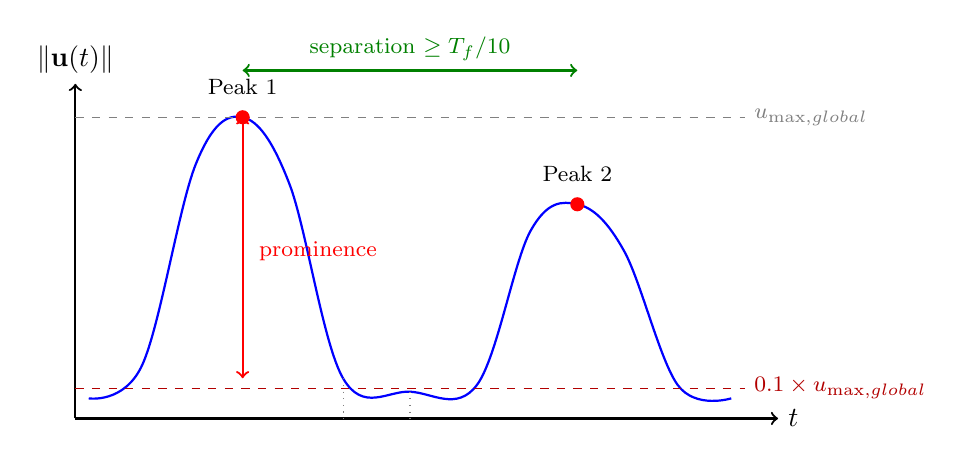
\begin{tikzpicture}[scale=0.85]
  % Axes
  \draw[->,thick] (0,0) -- (10.5,0) node[right] {$t$};
  \draw[->,thick] (0,0) -- (0,5.0) node[above] {$\|\mathbf{u}(t)\|$};
  % Thrust profile (synthetic bimodal)
  \draw[thick,blue] plot[smooth,tension=0.6] coordinates {
    (0.2,0.3) (1.0,0.8) (1.8,3.8) (2.5,4.5) (3.2,3.5) (4.0,0.6)
    (5.0,0.4) (6.0,0.5) (6.8,2.8) (7.5,3.2) (8.2,2.5) (9.0,0.5) (9.8,0.3)
  };
  % Global max dashed line
  \draw[dashed,gray] (0,4.5) -- (10,4.5);
  \node[gray,right] at (10,4.5) {\footnotesize $u_{\max,\text{global}}$};
  % 10% threshold line
  \draw[dashed,red!70!black] (0,0.45) -- (10,0.45);
  \node[red!70!black,right] at (10,0.45) {\footnotesize $0.1\times u_{\max,\text{global}}$};
  % Prominence arrow (peak 1)
  \draw[<->,thick,red] (2.5,0.6) -- (2.5,4.5);
  \node[red,right] at (2.6,2.5) {\footnotesize prominence};
  % Local minimum between peaks
  \draw[dotted,gray] (4.0,0.6) -- (4.0,0);
  \draw[dotted,gray] (5.0,0.4) -- (5.0,0);
  % Separation arrow
  \draw[<->,thick,green!50!black] (2.5,5.2) -- (7.5,5.2);
  \node[green!50!black,above] at (5.0,5.2) {\footnotesize separation $\geq T_f/10$};
  % Peak markers
  \fill[red] (2.5,4.5) circle (3pt);
  \fill[red] (7.5,3.2) circle (3pt);
  \node[above] at (2.5,4.7) {\footnotesize Peak 1};
  \node[above] at (7.5,3.4) {\footnotesize Peak 2};
\end{tikzpicture}
\caption{돌출도 기반 피크 탐지 기준의 개략도. 수직 화살표는 Peak~1의 돌출도(인접 극소값으로부터의 높이)를, 수평 화살표는 인접 피크 간 요구되는 최소 시간 간격을 나타낸다.}
\label{fig:peak_detection_schematic}
\end{figure}


%%%%%%%%%%%%%%%%%%%%%%%%%%%%%%%%%%%%%%%%%%%%%%%%%%%%%%%%%%%%%%%%%%
\section{결과: 추력 프로파일 데이터베이스}\label{sec:results_database}
%%%%%%%%%%%%%%%%%%%%%%%%%%%%%%%%%%%%%%%%%%%%%%%%%%%%%%%%%%%%%%%%%%

\subsection{데이터베이스 개요}\label{subsec:database_overview}

Section~\ref{subsec:configuration}에서 기술한 적응적 샘플링 전략을 네 개의 초기 고도 슬라이스($h_0 = 400$, 600, 800, 1000~km)에 독립적으로 적용하였다. Table~\ref{tab:db_summary}에 구축된 궤적 데이터베이스를 요약한다.

\begin{table}[ht]
\centering
\caption{궤적 데이터베이스 요약. [TBD: values to be updated after database regeneration with the expanded 5D configuration space.]}
\label{tab:db_summary}
\begin{tabular}{rrrrccc}
\hline
$h_0$ [km] & 전체 & 수렴 & 비율 & 단봉형 & 쌍봉형 & 다봉형 \\
\hline
400 & [TBD] & [TBD] & [TBD] & [TBD] & [TBD] & [TBD] \\
600 & [TBD] & [TBD] & [TBD] & [TBD] & [TBD] & [TBD] \\
800 & [TBD] & [TBD] & [TBD] & [TBD] & [TBD] & [TBD] \\
1000 & [TBD] & [TBD] & [TBD] & [TBD] & [TBD] & [TBD] \\
\hline
합계 & [TBD] & [TBD] & [TBD] & [TBD] & [TBD] & [TBD] \\
\hline
\end{tabular}
\end{table}

[TBD: convergence rate and statistics.] 미수렴 사례는 매개변수 공간의 경계 부근, 특히 요구 궤도요소 변화가 가용 전이 시간에 비해 큰 영역에서 집중적으로 발생할 것으로 예상된다. $T_f$가 자유 변수이고 완화된 수치 안전 장치 $u_{\max}$를 사용하는 현재 정식화에서는, 이전 정식화에서 미수렴의 원인이었던 물리적 추력 상한 $u_{\max}$ 초과와 달리, 주어진 전이 기간 범위 $[T_{\min}, T_{\max}]$가 요구 궤도 변화를 달성하기에 불충분한 경우가 미수렴의 주요 원인이다.

적응적 샘플링은 분류 경계 부근에 샘플을 효과적으로 집중시켰다(Fig.~\ref{fig:sampling_progress}). [TBD: entropy convergence statistics to be updated after database regeneration.]

\begin{figure}[ht]
\centering
\includegraphics[width=\columnwidth]{figures/fig7_sampling_progress.pdf}
\caption{각 초기 고도 슬라이스에 대한 적응적 샘플링 수렴 과정으로, 누적 평가 샘플 수를 나타낸다. [TBD: to be regenerated with 5D configuration space.]}
\label{fig:sampling_progress}
\end{figure}

\subsection{추력 프로파일 유형 분포}\label{subsec:type_distribution}

세 가지 추력 프로파일 유형---단봉형, 쌍봉형, 다봉형---을 데이터베이스에서 선정한 대표 사례를 통해 Fig.~\ref{fig:representative_profiles}에 예시한다.

\begin{figure*}[!htbp]
\centering
\includegraphics[width=\textwidth]{figures/fig1_representative_profiles.pdf}
\caption{각 분류 유형의 대표 추력 크기 프로파일: (a)~단일 추력 피크를 가진 단봉형, (b)~관성 비행 영역으로 분리된 두 개의 뚜렷한 추력 피크를 가진 쌍봉형, (c)~세 개 이상의 피크를 가진 다봉형. [To be regenerated: select clear examples with exactly 1, 2, and 3 peaks from the updated database.]}
\label{fig:representative_profiles}
\end{figure*}

단봉형 프로파일(Fig.~\ref{fig:representative_profiles}a)은 단일의 매끄러운 추력 피크를 나타내며, 하나의 궤도 위치에서 추진 노력을 집중한다. 이 패턴은 짧은 전이 기간에서 우세하며, 우주선이 다중 추력 아크를 형성할 충분한 시간이 없는 경우에 해당한다.

쌍봉형 프로파일(Fig.~\ref{fig:representative_profiles}b)은 거의 0에 가까운 추력의 관성 비행 영역으로 분리된 두 개의 뚜렷한 추력 피크를 보인다. 이 구조는 출발 및 도착 궤도 위치에서 추력이 집중되는 고전적 2-임펄스 호만 전이 기하에 직접 대응한다. [TBD: updated percentage of bimodal cases.]

다봉형 프로파일(Fig.~\ref{fig:representative_profiles}c)은 관성 비행 아크가 사이에 개재된 세 개 이상의 추력 피크를 나타낸다. 현재 데이터베이스는 단일 공전 미만 전이($T_f/T_0 \leq 1.2$)로 제한되므로, 다봉형 프로파일은 다중 공전 영역에 비해 발생 빈도가 낮을 것으로 예상되며, 주로 큰 고도-경사각-이심률 복합 변화에서 단일 궤도 공전 내에서도 다중 연소 전략이 에너지적으로 유리한 경우에 발생한다.

\begin{figure*}[!htbp]
\centering
\includegraphics[width=\textwidth]{figures/fig2_representative_trajectories.pdf}
\caption{Fig.~\ref{fig:representative_profiles}의 대표 프로파일에 대응하는 3차원 ECI 궤적: (a)~단봉형, (b)~쌍봉형, (c)~다봉형. [To be regenerated: increase point density, thicker trajectory lines, acceleration-proportional color mapping.]}
\label{fig:representative_trajectories}
\end{figure*}

대응하는 3차원 궤적을 Fig.~\ref{fig:representative_trajectories}에 나타낸다. 단봉형 사례(a)는 거의 직접적인 전이 아크를 보이며, 쌍봉형 사례(b)는 타원형 호만 궤도를 닮은 전이 기하를 나타낸다. 다봉형 사례(c)는 기하학적으로 유리한 궤도 위치에서 다수의 뚜렷한 추력 아크를 가진 단일 공전 미만 궤적을 보인다.

Table~\ref{tab:class_cost}에 각 프로파일 클래스별 $L^2$ 비용 통계를 요약한다. 비용 $J$의 단위는 km$^2$/s$^3$(가속도 제곱의 시간 적분)이다. 차원적으로, 특성 속도 변화 $\Delta v$를 기간 $T_f$ 동안 수행하는 전이의 경우 비용은 $J \sim (\Delta v)^2 / T_f$로 스케일링되며, 이는 기동 크기와 가용 전이 시간 간의 절충 관계를 반영한다.

\begin{table}[ht]
\centering
\caption{프로파일 클래스별 $L^2$ 비용 통계(수렴 사례만 포함). 비용 $J$의 단위는 km$^2$/s$^3$이다. [TBD: values to be updated after database regeneration.]}
\label{tab:class_cost}
\begin{tabular}{lrcccc}
\hline
클래스 & 수량 & 평균 $J$ & 표준편차 $J$ & 최솟값 $J$ & 최댓값 $J$ \\
 & & [km$^2$/s$^3$] & [km$^2$/s$^3$] & [km$^2$/s$^3$] & [km$^2$/s$^3$] \\
\hline
단봉형 & [TBD] & [TBD] & [TBD] & [TBD] & [TBD] \\
쌍봉형 & [TBD] & [TBD] & [TBD] & [TBD] & [TBD] \\
다봉형 & [TBD] & [TBD] & [TBD] & [TBD] & [TBD] \\
\hline
\end{tabular}
\end{table}

\subsection{지배 인자 분석}\label{subsec:dominant_factors}

추력 프로파일 분류에 가장 강하게 영향을 미치는 구성 매개변수를 식별하기 위해, 분류 맵과 GP 분류기의 ARD 커널 길이척도(ARD kernel length scale)를 분석한다.

\subsubsection{분류 맵}

Fig.~\ref{fig:classification_da_di}--\ref{fig:classification_di_T}에 각 고도 슬라이스에 대한 분류 경계의 2차원 투영을 나타낸다. 구성 공간이 5차원 $(\Delta a, \Delta i, e_0, e_f, T_f/T_0)$이므로, 각 2차원 맵은 나머지 세 매개변수를 대표값으로 고정하여 생성한다. [TBD: specify fixed values for each projection.] 이 맵들은 매개변수 공간에서 각 프로파일 유형과 관련된 영역을 보여준다.

\begin{figure*}[!htbp]
\centering
\includegraphics[width=\textwidth]{figures/fig3_classification_da_di.pdf}
\caption{각 초기 고도에 대한 $\Delta a$--$\Delta i$ 평면의 분류 맵: (a)~$h_0 = 400$~km, (b)~$h_0 = 600$~km, (c)~$h_0 = 800$~km, (d)~$h_0 = 1000$~km. [TBD: to be regenerated with 5D configuration space.]}
\label{fig:classification_da_di}
\end{figure*}

\begin{figure*}[!htbp]
\centering
\includegraphics[width=\textwidth]{figures/fig4_classification_da_T.pdf}
\caption{각 초기 고도에 대한 $\Delta a$--$T_f/T_0$ 평면의 분류 맵. [TBD: to be regenerated with 5D configuration space.]}
\label{fig:classification_da_T}
\end{figure*}

\begin{figure*}[!htbp]
\centering
\includegraphics[width=\textwidth]{figures/fig5_classification_di_T.pdf}
\caption{각 초기 고도에 대한 $\Delta i$--$T_f/T_0$ 평면의 분류 맵. [TBD: to be regenerated with 5D configuration space.]}
\label{fig:classification_di_T}
\end{figure*}

$\Delta a$--$T_f/T_0$ (Fig.~\ref{fig:classification_da_T}) 및 $\Delta i$--$T_f/T_0$ (Fig.~\ref{fig:classification_di_T}) 투영은 프로파일 유형 간 가장 명확한 분리를 나타내며, 전이 기간 $T_f/T_0$가 추력 프로파일 형태를 결정하는 지배적 인자임을 시사한다. 반면, $\Delta a$--$\Delta i$ 투영(Fig.~\ref{fig:classification_da_di})은 클래스 간 더 많은 중첩을 보여, 궤도요소 변화만으로는 프로파일 유형을 예측하기에 불충분함을 시사한다. [TBD: add projections involving $e_0$ and $e_f$.]

분류 맵의 3차원 시각화(Fig.~\ref{fig:classification_3d})는 분류 경계가 매개변수 공간에서 곡면을 형성하며, $T_f/T_0$가 분리의 주축을 제공함을 확인한다.

\begin{figure}[ht]
\centering
\includegraphics[width=\columnwidth]{figures/fig6_classification_3d.pdf}
\caption{$h_0 = 800$~km에 대한 3차원 분류 맵. [TBD: to be regenerated with 5D configuration space.]}
\label{fig:classification_3d}
\end{figure}

\subsubsection{ARD 길이척도 분석}

GP 분류기의 ARD 커널 길이척도는 분류가 각 입력 매개변수에 얼마나 민감하게 의존하는지를 정량화한다. 길이척도가 짧을수록 해당 차원을 따라 분류 함수가 더 빠르게 변하며, 이는 결과에 대한 더 강한 영향을 의미한다.

Table~\ref{tab:ard_lengthscales}에 각 고도 슬라이스별 ARD 길이척도를 제시한다. 확장된 5차원 구성 공간에 따라 두 개의 추가 길이척도 $\ell_{e_0}$와 $\ell_{e_f}$를 함께 보고한다.

\begin{table}[ht]
\centering
\caption{초기 고도별 ARD 길이척도. 작은 값은 분류에 대한 더 강한 영향을 나타낸다. [TBD: values to be updated after database regeneration.]}
\label{tab:ard_lengthscales}
\begin{tabular}{rccccc}
\hline
$h_0$ [km] & $\ell_{T_f/T_0}$ & $\ell_{\Delta a}$ & $\ell_{\Delta i}$ & $\ell_{e_0}$ & $\ell_{e_f}$ \\
\hline
400 & [TBD] & [TBD] & [TBD] & [TBD] & [TBD] \\
600 & [TBD] & [TBD] & [TBD] & [TBD] & [TBD] \\
800 & [TBD] & [TBD] & [TBD] & [TBD] & [TBD] \\
1000 & [TBD] & [TBD] & [TBD] & [TBD] & [TBD] \\
\hline
\end{tabular}
\end{table}

\begin{figure}[ht]
\centering
\includegraphics[width=\columnwidth]{figures/fig8_ard_lengthscales.pdf}
\caption{고도 슬라이스 간 ARD 길이척도 비교. [To be regenerated: use logarithmic scale for the ordinate to accommodate the large dynamic range, or consider removing if redundant with Table~\ref{tab:ard_lengthscales}.]}
\label{fig:ard_lengthscales}
\end{figure}

[TBD: ARD length scale analysis to be updated with five-dimensional results.] 무차원 전이 기간 $T_f/T_0$는 지배적 인자로 유지될 것으로 예상된다. 이심률 매개변수 $e_0$와 $e_f$의 $\Delta a$ 및 $\Delta i$ 대비 상대적 중요도는 단일 공전 미만 전이에서 궤도 형상이 추력 프로파일 형태 결정에 유의미한 역할을 하는지 여부를 밝혀줄 것이다.

고도 슬라이스 간 길이척도 순서의 일관성을 검토하여, 다섯 가지 구성 매개변수의 상대적 중요도가 초기 궤도 고도 선택에 대해 강건한지 여부를 판단할 것이다.

%%%%%%%%%%%%%%%%%%%%%%%%%%%%%%%%%%%%%%%%%%%%%%%%%%%%%%%%%%%%%%%%%%
\section{결과: 기하학적 분석}\label{sec:results_geometric}
%%%%%%%%%%%%%%%%%%%%%%%%%%%%%%%%%%%%%%%%%%%%%%%%%%%%%%%%%%%%%%%%%%

\subsection{형상 파라미터에 따른 비용 의존성}\label{subsec:cost_dependence}

Figure~\ref{fig:cost_vs_params}는 $L^2$ 비용을 각 형상 파라미터의 함수로 나타내며, 데이터 점은 프로파일 유형별로 색상을 구분하였다.

\begin{figure*}[!htbp]
\centering
\includegraphics[width=\textwidth]{figures/fig9_cost_vs_params.pdf}
\caption{형상 파라미터에 따른 $L^2$ 비용: (a)~$\Delta a$, (b)~$\Delta i$, (c)~$T/T_0$. 점은 프로파일 유형별로 색상을 구분하였다. [TBD: to be regenerated; add $e_0$, $e_f$ panels.]}
\label{fig:cost_vs_params}
\end{figure*}

몇 가지 경향이 관찰된다. 비용은 $|\Delta a|$와 $\Delta i$가 증가할수록 커지며, 이는 궤도요소 변화량이 클수록 더 큰 제어 노력이 필요하기 때문이다. $T_f/T_0$에 대한 의존성은 반비례 관계이다. 전이 기간이 길어지면 제어 노력을 더 긴 시간에 걸쳐 분산시킬 수 있어 최대 추력 요구량이 감소하고, 결과적으로 $L^2$ 비용이 줄어든다. 이 반비례 관계는 차원해석으로부터 예상되는 결과이다---고정된 궤도요소 변화에 대해 특성 제어 가속도는 $\Delta v / T_f$로 스케일링되며, $L^2$ 비용은 $(\Delta v)^2 / T_f$로 스케일링된다. [TBD: add scatter plots showing cost dependence on $e_0$ and $e_f$ as additional panels.]

프로파일 유형 또한 비용 크기와 상관관계를 보인다. 다봉형(multimodal) 프로파일은 더 높은 비용값에서 나타나는 경향이 있으며, 이는 보다 까다로운 전이 조건에 해당한다. 이는 단일 추력 호(thrust arc)로 필요한 궤도 변화를 에너지 예산 내에서 달성할 수 없을 때, 다중 임펄스(multi-impulse)와 유사한 전략이 나타나는 것과 일치한다.

\subsection{피크 시각 분석}\label{subsec:peak_timing}

추력 피크의 시간적 분포는 최적 추력 스케줄링을 지배하는 궤도역학적 메커니즘에 대한 통찰을 제공한다. Figure~\ref{fig:peak_timing}는 각 프로파일 유형별 정규화된 피크 시각($t_{\text{peak}} / T_f$)의 히스토그램을 나타낸다.

\begin{figure*}[!htbp]
\centering
\includegraphics[width=\textwidth]{figures/fig10_peak_timing.pdf}
\caption{프로파일 유형별 정규화된 피크 시각 분포: (a)~단봉형(unimodal), (b)~쌍봉형(bimodal), (c)~다봉형(multimodal). [TBD: to be regenerated with 5D configuration space.]}
\label{fig:peak_timing}
\end{figure*}

단봉형(unimodal) 프로파일(Fig.~\ref{fig:peak_timing}a)에서는 피크 시각이 전이 구간의 중간 지점($t/T_f \approx 0.5$) 부근에 집중되며, 이는 추력을 전이 중간 시점을 중심으로 대칭적으로 분배하는 에너지 최적 전략을 반영한다.

쌍봉형(bimodal) 프로파일(Fig.~\ref{fig:peak_timing}b)에서는 전이 시작과 끝 부근($t/T_f \approx 0$ 및 $t/T_f \approx 1$)에 두 개의 뚜렷한 군집이 나타나며, 이는 호만 전이(Hohmann transfer)의 두 임펄스에 대응하는 출발 및 도착 추력 호를 나타낸다.

다봉형(multimodal) 프로파일(Fig.~\ref{fig:peak_timing}c)에서는 중간 시점에 추가 피크가 나타나며, 이는 고도와 경사각 변화를 동시에 수행하기에 유리한 궤도 위치---일반적으로 궤도의 승교점 및 강교점 부근---에서 추력이 인가되는 것을 반영한다.


%%%%%%%%%%%%%%%%%%%%%%%%%%%%%%%%%%%%%%%%%%%%%%%%%%%%%%%%%%%%%%%%%%
\section{고찰}\label{sec:discussion}
%%%%%%%%%%%%%%%%%%%%%%%%%%%%%%%%%%%%%%%%%%%%%%%%%%%%%%%%%%%%%%%%%%

\subsection{지배 인자의 물리적 해석}\label{subsec:physical_interpretation}

[TBD: ARD length scale discussion to be updated with five-dimensional results.] ARD 길이척도 분석(Table~\ref{tab:ard_lengthscales})은 정규화된 전이 기간 $T_f/T_0$가 추력 프로파일 분류에 가장 영향력 있는 파라미터로 남을 것으로 예상된다. 이 결과는 궤도역학에 기반한 명확한 물리적 설명을 갖는다.

데이터베이스가 단일 공전 미만 전이($T_f/T_0 \leq 1.2$)로 제한되므로, 우주선은 최대 1.2 궤도 회전을 완료한다. 이 범위 내에서 최적화기는 다중 추력 호의 스케줄링에 제한된 유연성을 가지며, 에너지 최적 전략은 추진 노력을 하나 또는 두 개의 연속 연소에 집중시켜 주로 단봉형 또는 쌍봉형 프로파일을 산출한다. 다봉형 프로파일은 다중 회전 데이터베이스에 비해 덜 빈번하게 발생할 것으로 예상되며, 주로 장반경, 경사각, 이심률의 대규모 복합 변화를 요구하는 전이에서 나타난다.

장반경 변화 $\Delta a$는 총 에너지 요구량을 결정하며, 이는 쌍봉형 해가 최적이 되는 임계 기간을 조절한다. 경사각 변화 $\Delta i$는 주로 추력 방향(면외 성분)에 영향을 미치며, 추력 호의 개수에는 약한 영향을 미친다. 이심률 파라미터 $e_0$와 $e_f$의 역할은 특히 주목할 만하다. 비영(non-zero) 이심률은 궤도를 따라 중력장에 근-원점(apsidal) 비대칭을 도입하며, 이는 근지점 또는 원지점 부근에서 기하학적으로 유리한 추력 위치를 생성하여 피크 구조에 영향을 미칠 수 있다.

\subsection{임펄스 기동과의 대응 관계}\label{subsec:impulsive_correspondence}

Section~\ref{subsec:impulsive_relation}의 이론적 프레임워크는 연속 추력 프로파일이 고전적 임펄스 기동과 구조적 대응 관계를 보여야 한다고 예측한다. 데이터베이스 결과는 이 예측을 정량적으로 확인한다.

쌍봉형(bimodal) 프로파일은 두 개의 뚜렷한 추력 집중 영역을 특징으로 하며, 2-임펄스 전이의 연속 추력 대응물(analog)을 나타낸다. 두 추력 피크는 출발 및 도착 궤도 위치 부근에서 발생하며, 순간적으로 인가되었을 속도 변화를 부드럽게 분배한다. 궤도요소 $(a_0, e_0)$와 $(a_f, e_f)$를 갖는 궤도 간의 일반적인 2-임펄스 전이에 대해, 총 임펄스 $\Delta v$는 전이 궤도 기하구조에 의존한다. 동일 평면 원궤도($e_0 = e_f = 0$) 사이의 전이라는 특수한 경우에 이는 고전적 호만 $\Delta v$로 축소된다:
\begin{equation}\label{eq:hohmann_dv}
\Delta v_H = \left|\sqrt{\frac{\mu}{a_0}}\left(\sqrt{\frac{2a_f}{a_0+a_f}} - 1\right)\right| + \left|\sqrt{\frac{\mu}{a_f}}\left(1 - \sqrt{\frac{2a_0}{a_0+a_f}}\right)\right|
\end{equation}
타원궤도의 경우 임펄스 $\Delta v$는 출발 및 도착 궤도의 근지점/원지점 속도를 고려하여 Lambert 문제 정식화를 통해 수치적으로 계산된다. [TBD: generalized $\Delta v$ computation for eccentric orbit transfers.]

Figure~\ref{fig:hohmann_correspondence}는 이 임펄스 $\Delta v$를 데이터베이스 내 모든 수렴 사례의 $L^2$ 비용과 비교한다.

\begin{figure}[ht]
\centering
\includegraphics[width=\columnwidth]{figures/fig11_hohmann_correspondence.pdf}
\caption{호만(Hohmann) $\Delta v$ 대 연속 추력 $L^2$ 비용. 프로파일 유형별로 색상을 구분하였다. [TBD: to be regenerated with 5D configuration space including eccentric orbits.]}
\label{fig:hohmann_correspondence}
\end{figure}

[TBD: correlation analysis to be updated with the expanded database including eccentric orbits.] 데이터베이스 결과는 쌍봉형 사례가 임펄스 $\Delta v$와 $L^2$ 비용 사이에 양의 상관관계를 나타낼 것으로 예상된다. 순수 고도 변경 사례($\Delta i = 0$, $e_0 = e_f = 0$)에서 비율 $J_{L^2} / (\Delta v_H)^2$는 $T_f/T_0$에 의존하는 상수에 수렴해야 하며, 이는 짧은 기간 극한에서 연속 추력 비용이 임펄스 비용에 수렴한다는 스케일링 논거와 일치한다.

단일 공전 미만 범위 내에서 다봉형 프로파일은 기하학적으로 유리한 궤도 위치에서 추가 추력 호를 활용하는 다중 연소 전략에 대응한다. 제한된 전이 기간($T_f/T_0 \leq 1.2$)은 이중 타원형(bi-elliptic) 기동의 범위를 제한하므로, 다봉형 프로파일은 주로 다수의 궤도요소에 대한 대규모 복합 변화를 수반하는 전이에서 발생할 것으로 예상된다.

\subsection{실용적 시사점}\label{subsec:practical_implications}

분류 맵과 지배 인자 분석은 임무 설계자에게 몇 가지 실용적 도구를 제공한다.

첫째, 분류 맵(Figs.~\ref{fig:classification_da_di}--\ref{fig:classification_di_T})은 재사용 우주비행체(ReUSV) 및 군집위성(constellation) 임무에 대해 예상되는 추력 프로파일 구조의 신속한 평가를 가능하게 한다. 설계자는 이 맵을 참조하여 주어진 전이가 단봉형, 쌍봉형, 또는 다봉형 해를 산출할 가능성이 높은지를 전체 최적화 문제를 풀지 않고 판단할 수 있다. 이 기능은 많은 후보 형상을 효율적으로 선별해야 하는 예비 임무 설계 단계에서 특히 유용하다.

둘째, $T_f$를 단일 공전 미만 범위 내의 자유 변수로 취급함으로써 임무 설계자에게 실용적 프레임워크를 제공한다. 주어진 전이 기하구조(타원궤도 포함)에 대해 최적화기가 에너지적으로 최적인 전이 기간을 결정하며, 그 결과의 추력 프로파일 유형이 기동 복잡성을 나타낸다. [TBD: identify the $T_f/T_0$ threshold separating unimodal from bimodal within the sub-single-revolution regime.]

셋째, 임펄스 $\Delta v$와 $L^2$ 비용 사이의 정량적 대응 관계는 고전적 임펄스 해로부터 연속 추력 비용의 신속한 추정을 가능하게 하여, 예비 임펄스 설계와 상세 연속 추력 최적화 사이의 간극을 연결한다. 이는 특히 신속한 궤도 복귀 일정이 가용 전이 기간을 제약하는 ReUSV 임무 계획에 유용하다.

\subsection{한계 및 향후 연구}\label{subsec:limitations}

본 연구는 향후 연구 방향을 시사하는 몇 가지 한계를 갖는다.

첫째, 근지점 편각 $\omega$는 출발 및 도착 궤도 모두에서 0으로 고정된다. 타원궤도의 경우 장축 방향(apse line)이 추력 호의 상대 기하구조에 영향을 미치므로, $\omega$를 자유 파라미터로 포함하면 이 효과를 포착하기 위해 구성 공간이 확장될 것이다.

둘째, 동역학 모델에는 $J_2$ 섭동만 포함된다. $J_2$가 LEO에서 지배적이지만, 약 500~km 고도 미만에서는 대기 항력이 유의해지며, 수일 이상 지속되는 전이에서는 태양 및 달의 제3체 효과가 영향을 미칠 수 있다. 이러한 효과를 포함하면 특정 임무 시나리오에 대한 충실도가 향상될 것이다.

셋째, $L^1$(연료 최적) 정식화 대신 $L^2$(에너지 최적) 비용함수를 사용한다. $L^2$ 노름은 본질적인 피크 구조를 보존하지만, 결과 프로파일은 연료 최적 대응물보다 부드럽다. $L^1$ 노름 하의 뱅-뱅(bang-bang) 제어 프로파일로 분석을 확장하면 임펄스 전환 구조와의 직접적 대응을 제공할 것이다.

넷째, 데이터베이스는 단일 공전 미만 전이($T_f/T_0 \leq 1.2$)로 제한된다. 다중 회전 전이로 확장하면 분류 경관을 완성하고, 추력 스케줄링에 더 많은 궤도 회전이 가용해짐에 따라 경계가 어떻게 진화하는지를 드러낼 것이다.

다섯째, 직접 배치법(direct collocation)은 국소 최적해를 구하며, 전역 최적성은 보장되지 않는다. 웜 스타팅(warm-starting)을 포함한 2-패스 접근법이 이 문제를 완화하지만, 특히 다수의 추력 스케줄링 전략이 공존하는 다봉형 영역에서 일부 사례는 차선의 국소 최솟값에 수렴할 수 있다.

마지막으로, 현재 분류는 추력 피크의 개수에만 기반한다. 피크 진폭 비, 시간 간격, 활주 호(coasting arc) 지속 시간을 포함하는 보다 정교한 분류 체계는 전이 기하구조와 최적 추력 구조 사이의 관계에 대한 추가적 통찰을 제공할 수 있을 것이다.


%%%%%%%%%%%%%%%%%%%%%%%%%%%%%%%%%%%%%%%%%%%%%%%%%%%%%%%%%%%%%%%%%%
\section{결론}\label{sec:conclusions}
%%%%%%%%%%%%%%%%%%%%%%%%%%%%%%%%%%%%%%%%%%%%%%%%%%%%%%%%%%%%%%%%%%

본 연구는 재사용 우주비행체(ReUSV) 운용과 LEO 군집위성 관리의 궤적 설계 필요성에 의해 동기부여된, LEO-to-LEO 전이 임무에 대한 최적 연속 추력 프로파일의 체계적 파라메트릭 분석을 수행하였다. CasADi와 IPOPT로 구현된 2-패스 직접 배치법(direct collocation)을 사용하여 포괄적인 최적 궤적 데이터베이스를 구축하였으며, 장반경 변화, 경사각 변화, 출발 이심률, 도착 이심률, 전이 기간의 5차원 구성 공간에 걸쳐 네 개의 초기 고도 슬라이스($h_0 = 400$, 600, 800, 1000~km)를 다루었다. 전이 기간은 단일 공전 미만 범위($T_f/T_0 \leq 1.2$) 내의 자유 최적화 변수로 취급하였다.

주요 연구 결과를 요약하면 다음과 같다:

\begin{enumerate}
\item [TBD: database size, convergence rate, and class distribution statistics.] 추력 프로파일은 단봉형(unimodal), 쌍봉형(bimodal), 다봉형(multimodal)의 세 가지 뚜렷한 유형으로 분류된다. 다봉형 프로파일은 제한된 전이 기간으로 인해 다중 회전 데이터베이스에 비해 덜 빈번하게 발생할 것으로 예상된다.

\item [TBD: ARD length scale analysis with five parameters.] 정규화된 전이 기간 $T_f/T_0$는 추력 프로파일 형태를 지배하는 주요 인자로 남을 것으로 예상된다. 이심률 파라미터 $e_0$와 $e_f$의 상대적 중요도는 최적 추력 스케줄 결정에서 궤도 형상의 역할을 정량화할 것이다.

\item 분류 경계는 네 개의 고도 슬라이스에 걸쳐 검토되며, 정규화된 파라미터화가 LEO 고도 범위 전반에 걸쳐 본질적 물리를 포착하는지를 평가한다.

\item 연속 추력 프로파일 유형과 고전적 임펄스 기동 사이의 정량적 대응 관계가 확립되며, 수치적 $\Delta v$ 계산을 통해 타원궤도 전이를 포함하도록 일반화된다.
\end{enumerate}

이러한 결과는 임무 설계자에게 전이 기하구조만으로 최적 추력 프로파일 특성을 예측할 수 있는 지침을 제공하며, ReUSV 궤도 복귀 및 랑데부 임무 계획을 위한 신속한 예비 평가를 가능하게 한다. 분류 프레임워크와 데이터베이스는 다중 회전 전이, 근지점 편각의 추가 자유 파라미터화, 고충실도 동역학 모델, 연료 최적 정식화로의 향후 확장을 위한 기반을 제공한다.


%%%%%%%%%%%%%%%%%%%%%%%%%%%%%%%%%%%%%%%%%%%%%%%%%%%%%%%%%%%%%%%%%%
%% Acknowledgments
%%%%%%%%%%%%%%%%%%%%%%%%%%%%%%%%%%%%%%%%%%%%%%%%%%%%%%%%%%%%%%%%%%
\section*{Acknowledgments}
This work was supported by Korea Research Institute for defense Technology planning and advancement (KRIT) grant funded by the Korea government (DAPA (Defense Acquisition Program Administration)) (No. KRIT-CT-22-030, ReUSV-41, 2025).


%%%%%%%%%%%%%%%%%%%%%%%%%%%%%%%%%%%%%%%%%%%%%%%%%%%%%%%%%%%%%%%%%%
%% Appendix
%%%%%%%%%%%%%%%%%%%%%%%%%%%%%%%%%%%%%%%%%%%%%%%%%%%%%%%%%%%%%%%%%%
\appendix
\section{가우시안 프로세스 능동 샘플링}\label{app:gp_sampling}

본 부록에서는 적응적 데이터베이스 구축에 사용된 가우시안 프로세스(Gaussian Process, GP) 분류 프레임워크와 엔트로피 기반 능동 샘플링 전략의 수학적 세부 사항을 제공한다.

\subsection{다중 클래스 가우시안 프로세스 분류}

가우시안 프로세스 분류는 연결 함수(link function)의 도입을 통해 GP 회귀 프레임워크를 범주형 출력으로 확장한다. 본 연구에서 고려하는 $C = 3$ 클래스 문제에 대해 소프트맥스(softmax, 다항 로지스틱) 우도를 사용한다.

각 클래스 $c \in \{0, 1, 2\}$에 대해 잠재 함수 $f_c: \mathcal{X} \rightarrow \mathbb{R}$를 도입한다. 집합 $\mathbf{f}(\mathbf{x}) = (f_0(\mathbf{x}), f_1(\mathbf{x}), f_2(\mathbf{x}))^\top$은 독립적인 가우시안 프로세스로 모델링된다:
\begin{equation}
f_c(\mathbf{x}) \sim \mathcal{GP}(0, k(\mathbf{x}, \mathbf{x}'))
\end{equation}

클래스 확률은 소프트맥스 변환을 통해 얻어진다:
\begin{equation}\label{eq:softmax}
p(y = c \mid \mathbf{x}, \mathbf{f}) = \frac{\exp(f_c(\mathbf{x}))}{\sum_{j=0}^{2} \exp(f_j(\mathbf{x}))}
\end{equation}

잠재 함수의 공분산 구조는 커널 함수 $k(\mathbf{x}, \mathbf{x}')$를 통해 지정된다. 본 연구에서는 자동 관련성 결정(Automatic Relevance Determination, ARD) 제곱지수 커널을 채택한다:
\begin{equation}\label{eq:ard_kernel}
k(\mathbf{x}, \mathbf{x}') = \sigma_f^2 \exp\left(-\frac{1}{2} \sum_{d=1}^{D} \frac{(x_d - x_d')^2}{\ell_d^2}\right)
\end{equation}
여기서 $D = 5$는 구성 파라미터 $(\Delta a, \Delta i, e_0, e_f, T_f/T_0)$의 수이며, $\sigma_f^2$는 함수 변동의 크기를 제어하는 신호 분산이고, $\ell_d$는 각 입력 차원의 특성 길이척도이다. ARD 구조는 모델이 분류 결과 결정에서 각 파라미터의 상대적 중요도를 학습할 수 있게 한다. 작은 길이척도는 해당 파라미터가 분류에 강하게 영향을 미침을 나타내며, 큰 길이척도는 약한 의존성을 시사한다.

훈련 데이터셋 $\mathcal{D} = \{(\mathbf{x}_i, y_i)\}_{i=1}^{N}$가 주어지면, 비가우시안 우도로 인해 잠재 함수에 대한 사후분포는 해석적으로 구할 수 없다. 본 연구에서는 사후분포를 최대 사후 확률(MAP) 추정치를 중심으로 한 가우시안 분포로 근사하는 라플라스 근사를 사용한다:
\begin{equation}
p(\mathbf{f} \mid \mathcal{D}) \approx \mathcal{N}(\mathbf{f} \mid \hat{\mathbf{f}}, \mathbf{A}^{-1})
\end{equation}
여기서 $\hat{\mathbf{f}} = \arg\max_{\mathbf{f}} p(\mathbf{f} \mid \mathcal{D})$이고, $\mathbf{A} = -\nabla\nabla \log p(\mathbf{f} \mid \mathcal{D})|_{\mathbf{f}=\hat{\mathbf{f}}}$는 음의 로그 사후분포의 헤시안(Hessian)이다.

초파라미터 벡터 $\boldsymbol{\theta} = (\sigma_f, \ell_1, \ldots, \ell_D)$는 관측 데이터의 주변 우도를 최대화하여 추정한다.

\subsection{엔트로피 기반 획득 함수}

능동 샘플링의 목표는 분류 함수에 대한 기대 정보 이득을 최대화하는 다음 질의 점 $\mathbf{x}_{N+1}$을 선택하는 것이다. 정보이론적 관점에서 이는 예측 분포의 엔트로피를 최대한 줄이는 점을 선택하는 것에 해당한다.

후보 점 $\mathbf{x}$에서의 예측 엔트로피는 클래스 예측의 불확실성을 정량화한다:
\begin{equation}\label{eq:entropy}
H[p(y \mid \mathbf{x}, \mathcal{D})] = -\sum_{c=0}^{2} p(y = c \mid \mathbf{x}, \mathcal{D}) \log p(y = c \mid \mathbf{x}, \mathcal{D})
\end{equation}

엔트로피는 세 클래스가 모두 동일한 확률일 때 최댓값 $\log 3 \approx 1.099$를 달성하며, 이는 최대 불확실성을 나타낸다. 반대로 분류기가 단일 클래스에 대해 확신할 때 엔트로피는 0에 접근한다.

엔트로피 기반 능동 샘플링의 획득 함수는 단순히 예측 엔트로피이다:
\begin{equation}
\alpha(\mathbf{x}) = H[p(y \mid \mathbf{x}, \mathcal{D})]
\end{equation}

다음 샘플 위치는 후보 집합에 대해 이 획득 함수를 최대화하여 선택된다:
\begin{equation}
\mathbf{x}_{N+1} = \arg\max_{\mathbf{x} \in \mathcal{X}_{\text{cand}}} \alpha(\mathbf{x})
\end{equation}

이 선택 기준은 직관적 해석을 갖는다. 높은 예측 엔트로피를 갖는 점들은 분류기가 불확실한 결정 경계 근처에 위치하며, 이러한 위치에서의 샘플링은 경계 추정을 정밀화하는 데 가장 많은 정보를 제공한다.

\subsection{샘플링 알고리즘}

전체 샘플링 절차는 두 단계로 구성된다. 전역 커버리지를 확보하기 위한 초기 공간 충전 단계와, 결정 경계 근처에 샘플을 집중시키는 적응 단계이다.

\textbf{1단계: 초기 커버리지.} 라틴 초입방체 샘플링(Latin Hypercube Sampling, LHS)으로 $N_{\text{init}} = 100$개의 초기 샘플 집합을 생성한다. LHS는 각 좌표를 $N_{\text{init}}$개의 동일 구간으로 나누고 각 구간에 정확히 하나의 샘플을 배치하여, 다차원 상관관계를 무작위화하면서 각 차원의 균일한 커버리지를 보장한다.

\textbf{2단계: 적응 샘플링 루프.} 적응 샘플링은 다음과 같이 진행된다:

\begin{enumerate}
\item 주변 우도 최대화를 통해 초파라미터를 최적화하여 현재 데이터셋 $\mathcal{D}$에 대해 GP 분류기를 훈련한다.

\item 각 후보 점 $\mathbf{x} \in \mathcal{X}_{\text{cand}}$에 대해 예측 엔트로피 $\alpha(\mathbf{x})$를 계산한다.

\item $\max_{\mathbf{x}} \alpha(\mathbf{x}) < \varepsilon$ (수렴 임계값)이면 종료한다.

\item $\mathbf{x}^* = \arg\max_{\mathbf{x}} \alpha(\mathbf{x})$를 선택한다.

\item $\mathbf{x}^*$에서 궤적 최적화 문제를 풀어 클래스 레이블 $y^*$를 얻는다.

\item 데이터셋을 확장한다: $\mathcal{D} \leftarrow \mathcal{D} \cup \{(\mathbf{x}^*, y^*)\}$.

\item 샘플 수가 $N_{\text{update}}$의 배수이면 GP 초파라미터를 재최적화한다.

\item $|\mathcal{D}| \geq N_{\max}$가 될 때까지 2단계부터 반복한다.
\end{enumerate}

후보 집합 $\mathcal{X}_{\text{cand}}$는 5차원 정규화된 파라미터 공간에서 무작위로 샘플링된 점으로 구성된다($|\mathcal{X}_{\text{cand}}| = 50{,}000$). 5차원에 대한 정규 격자는 비현실적으로 크기 때문이다. 수렴 임계값은 $\varepsilon = 0.3$으로 설정하며, 이는 가장 가능성 높은 클래스에 대해 약 85\% 신뢰도에 해당한다.

계산 효율성을 위해 배치 샘플링은 다양성 제약 $\|\mathbf{x}_i - \mathbf{x}_j\| \geq d_{\min}$ ($i \neq j$인 모든 쌍에 대해)을 적용하여 가장 높은 엔트로피를 갖는 $k$개의 점을 선택하며, 중복되는 인접 점의 선택을 방지한다. 본 연구에서는 배치 크기 $k = 10$, 정규화 좌표에서의 최소 간격 $d_{\min} = 0.1$을 사용한다.

% To print the credit authorship contribution details
\printcredits

%% Loading bibliography style file
%\bibliographystyle{model1-num-names}
\bibliographystyle{cas-model2-names}

% Loading bibliography database
\bibliography{cas-refs}

% Biography
%\bio{}
% Here goes the biography details.
%\endbio

%\bio{pic1}
% Here goes the biography details.
%\endbio

\end{document}
